\section{Evaluation}
\label{sec:evaluation}

Two standard metrics are used to measure the accuracy of link mining algorithms: AUC and  \textit{Precision} \cite{Lu2011}. We focused here on AUC because it is stronger in revealing false positivity issues.

The original dataset is partitioned into a trainset and a testset, according to a test ratio. Both the dataset and the trainset are made of one single giant connected component.

We recall here the AUC definition:

\begin{equation}
\label{eqn:auc}
AUC=\frac{n_{1}+0.5n_{2}}{n}
\end{equation}

where 
$n_{1}$ is the number of times a missing link has a score greater than an inexistent link,
$n_{2}$ is the number of times a missing link has a score equal to an inexistent link and
$n$ is the total number of combination of missing links and inexistent links.

Our experimental framework consists in measuring the AUC for all classical and novel metrics, applied to both criminal and not criminal datasets with test ratios at 10\% and 15\%.
In particular, we analyze the giant component of
(i) a criminal dataset (CRM) collecting wiretrap-records, judgement and arrest warrants \cite{berlusconi2016link}; and
(ii) a business-related dataset (BSN) collecting face-to-face interactions between employees in a IT company \cite{olguin2009sensible}.

In Table~\ref{tab:auc-detection} and \ref{tab:auc-prediction} we listed results for link detection and prediction, respectively, highlighting the most notable ones.

%\begin{figure}[!ht]
%	\centering
%	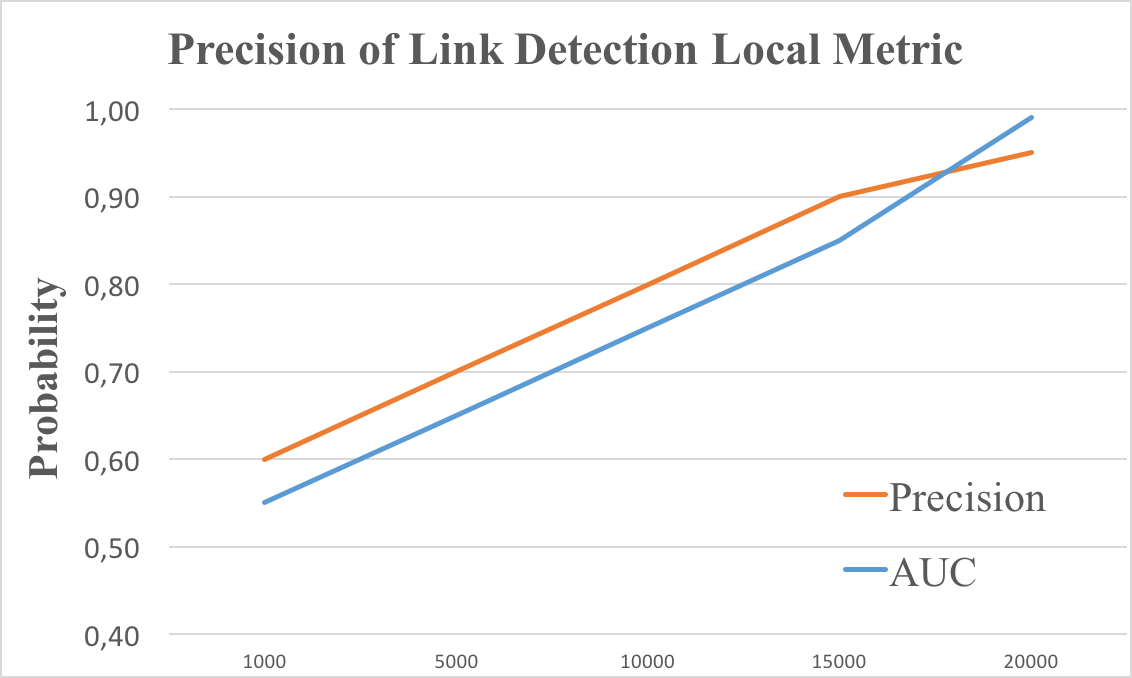
\includegraphics[width=0.48\textwidth]{graphs/graph_detection.png}
%	\caption{Precision of local metric for link detection}
%	\label{fig:graph-detection}
%\end{figure}

%\begin{figure}[!ht]
%	\centering
%	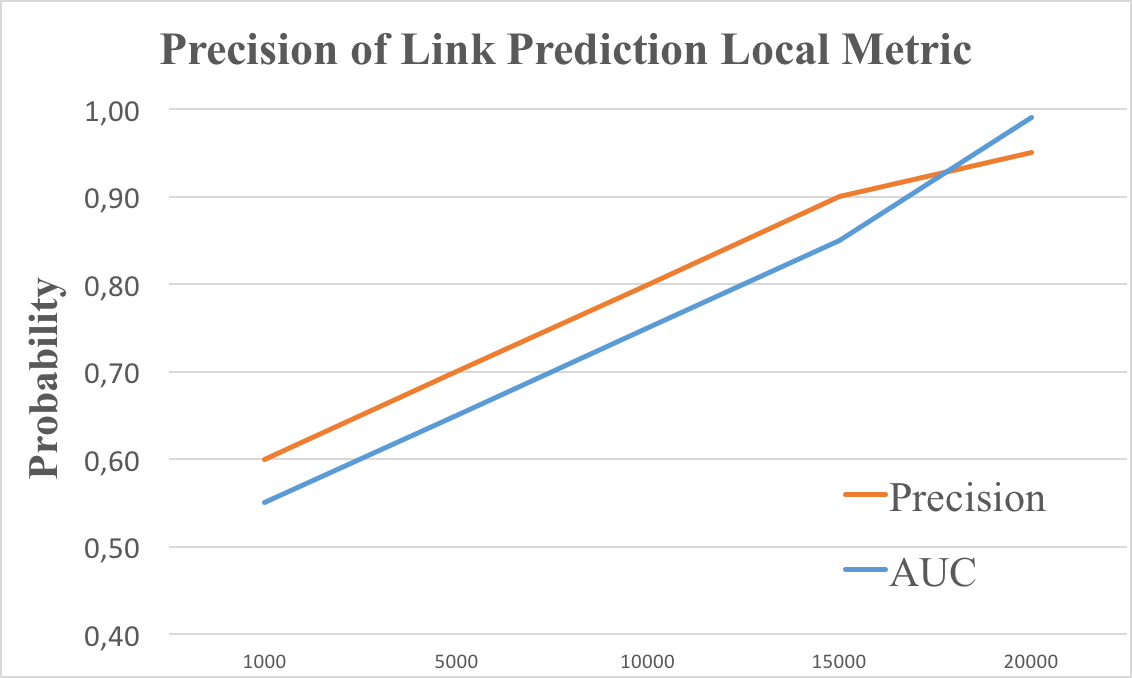
\includegraphics[width=0.48\textwidth]{graphs/graph_prediction.png}
%	\caption{Precision of local metric for link prediction}
%	\label{fig:graph-prediction}
%\end{figure}

\begin{table}[h]
	\centering
	\begin{tabular}{l l l l l}
	\toprule
	\textbf{Metric} & \textbf{CRM-10} & \textbf{CRM-15} & \textbf{RND-10} & \textbf{RND-15}\\\\
	\midrule
		Common Neighbours & $0.99$ & $0.99$ & $0.99$ & $0.99$ \\
		Salton  & $0.99$ & $0.99$ & $0.99$ & $0.99$ \\
		Jaccard  & $0.99$ & $0.99$ & $0.99$ & $0.99$ \\
		Sorensen   & $0.99$ & $0.99$ & $0.99$ & $0.99$ \\
		Hub Promoted  & $0.99$ & $0.99$ & $0.99$ & $0.99$ \\
		Hub Depressed  & $0.99$ & $0.99$ & $0.99$ & $0.99$ \\
		Leicht-Holme-Newman  & $0.99$ & $0.99$ & $0.99$ & $0.99$ \\
		Preferential Attachment  & $0.99$ & $0.99$ & $0.99$ & $0.99$ \\
		Adamic-Adar  & $0.99$ & $0.99$ & $0.99$ & $0.99$ \\
		Resource Allocation (RA)  & $0.99$ & $0.99$ & $0.99$ & $0.99$ \\
		Normalized RA  & $0.99$ & $0.99$ & $0.99$ & $0.99$ \\
		Traffic Allocation  & $0.99$ & $0.99$ & $0.99$ & $0.99$ \\
		Normalized TA  & $0.99$ & $0.99$ & $0.99$ & $0.99$ \\
	\bottomrule
	\end{tabular}
	\label{tab:auc-detection}
	\caption{AUC for Detection.}
\end{table}

\begin{table}[h]
	\centering
	\begin{tabular}{l l l l l}
	\toprule
	\textbf{Metric} & \textbf{CRM-10} & \textbf{CRM-15} & \textbf{RND-10} & \textbf{RND-15}\\\\
	\midrule
		Common Neighbours & $0.99$ & $0.99$ & $0.99$ & $0.99$ \\
		Salton  & $0.99$ & $0.99$ & $0.99$ & $0.99$ \\
		Jaccard  & $0.99$ & $0.99$ & $0.99$ & $0.99$ \\
		Sorensen   & $0.99$ & $0.99$ & $0.99$ & $0.99$ \\
		Hub Promoted  & $0.99$ & $0.99$ & $0.99$ & $0.99$ \\
		Hub Depressed  & $0.99$ & $0.99$ & $0.99$ & $0.99$ \\
		Leicht-Holme-Newman  & $0.99$ & $0.99$ & $0.99$ & $0.99$ \\
		Preferential Attachment  & $0.99$ & $0.99$ & $0.99$ & $0.99$ \\
		Adamic-Adar  & $0.99$ & $0.99$ & $0.99$ & $0.99$ \\
		Resource Allocation (RA)  & $0.99$ & $0.99$ & $0.99$ & $0.99$ \\
		Normalized RA  & $0.99$ & $0.99$ & $0.99$ & $0.99$ \\
		Traffic Allocation (TA)  & $0.99$ & $0.99$ & $0.99$ & $0.99$ \\
		Normalized TA  & $0.99$ & $0.99$ & $0.99$ & $0.99$ \\
	\bottomrule
	\end{tabular}
	\label{tab:auc-prediction}
	\caption{AUC for Precision.}
\end{table}	

The experimental results show that classic metrics achieve great performance in prediction tasks, while the novel metrics do it in detection.
In particular, we notice that in prediction some metrics are clearly distinct from others froma performance point of view; while in detection they are all similar.



     
%\begin{figure}
%	\centering
%	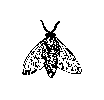
\includegraphics{./fig/fly}
%	\caption{AUC and Precision indices for link detection metric, considering both a criminal and a social network dataset.}
%	\label{fig:performance-detection}
%\end{figure}

%\begin{figure}
%	\centering
%	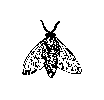
\includegraphics{./fig/fly}
%	\caption{AUC and Precision indices for link prediction metric, considering both a criminal and a social network dataset.}
%	\label{fig:performance-prediction}
%\end{figure}

% DA INSERIRE
%Formally, for two istants $t$ and $t' > t$, we denote $G[t,t']$ the subgraph of G consisting of all edges with a timestamp between $t$ and $t'$. Identified four times: $t_{0}, t'_{0}, t_{1}, t''_{1}$, with $t_{0}<t'_{0}<t_{1}<t'_{1}$, we refer to $[t_{0},t'_{0}]$ as the \textit{training interval} and $[t_{1},t'_{1}]$ as the \textit{test interval}. Applying a \textit{prediction algorithm} on the graph obtained after the training interval, as $G[t_{0},t'_{0}]$, we want to make a prediction on the edges that will be present in the graph $G[t_{1},t'_{1}]$ and not present in $G[t_{0},t'_{0}]$\cite{Liben-Nowell}.
%In this work, the notions of training interval and test interval, are provided with the only purpose to test the algorithm that will be presented in the following. After all, this application produce an output of links mining in real time: in which each instant $t\textsuperscript{*}>t_{0}$ identifies a graph $G[t_{0},t\textsuperscript{*}]$ on which to execute the algorithm. More details about the real time processing are explained in Section \ref{sec:architecture}.

%Notice that, in this work we assume that the graph is connected, therefore each pair of nodes is connected by a path. If we had in the case of a not connected graph, with a large connected component, as \textit{giant component}, and other small size connected components, the accuracy would be distorted by different \textit{density} of edges in a connected components.